\documentclass{beamer}

\usetheme{hpl1}
\usecolortheme{default}
% fine for B/W printing:
%\usecolortheme{seahorse}

%\usefonttheme{}
%\useinntertheme{}
%\useoutertheme{}

\usepackage{pgf,pgfarrows,pgfnodes,pgfautomata,pgfheaps,pgfshade}
\usepackage{graphicx}
%\usepackage{epsfig}
\usepackage{fancyvrb,moreverb,relsize}
\usepackage{amsmath,amssymb}
\usepackage[latin1]{inputenc}
\usepackage{colortbl}
\usepackage[english]{babel}

% Use some nice templates
\beamertemplatetransparentcovereddynamic

% User's newcommands:
\newcommand{\emp}[1]{{\smaller\texttt{#1}}}
\newcommand{\mathbfx}[1]{{\mbox{\boldmath $#1$}}}
\newcommand{\OBS}[1]{\marginpar{\scriptsize##1}}

\begin{document}

\title{GPH 483/598 Geographic Information Analysis}

\author[Rey]{Sergio J. Rey}

\institute{GeoDa Center for Gecomputation and Spatial Analysis
\and
School of Geographical Sciences and Urban Planning,
\and
Arizona State University}

\date{Spring 2010 \\ \ \\
\centerline{\psfig{figure=wave-dueto-slide.ps,width=0.5\linewidth}}
}

% Delete this, if you do not want the table of contents to pop up at
% the beginning of each section:
\AtBeginSection[]
{
    \begin{frame}<beamer>[plain]
    \frametitle{List of Topics}
    \tableofcontents[currentsection]
    \end{frame}
}

% Delete this, if you do not want the table of contents to pop up at
% the beginning of each subsection:
\AtBeginSubsection[]
{
    \begin{frame}<beamer>[plain]
    \frametitle{List of Topics}
    \tableofcontents[currentsection,currentsubsection]
    \end{frame}
}

% If you wish to uncover everything in a step-wise fashion, uncomment
% the following command: 

%\beamerdefaultoverlayspecification{<+->}

\begin{frame}
\titlepage
\end{frame}

% table of contents:
\begin{frame}[plain]
\frametitle{List of Topics}

\begin{columns}

\column{0.5\textwidth}
\tableofcontents
%\tableofcontents[pausesections]

\column{0.5\textwidth}
\begin{center}
\psfig{figure=python1.ps,width=1\linewidth}
\end{center}

\end{columns}
\end{frame}

\section[Intro]{Intro to Latexslides}


\subsection[Objectives]{Objectives}


\begin{frame}
\frametitle{Course Objectives}

\begin{block}

\begin{itemize}
\item<2,5> Introduce fundamentals of ESDA
\item<3,5> Conceptual and theoretical background
\item<4,5> Hands-on experience
\end{itemize}

\end{block}

\end{frame}

\subsection[Components]{Components}


\begin{frame}
\frametitle{Components}

\begin{block}{Four Sections:}

\begin{itemize}
\item<2,6> Introduction to Spatial Data
\item<3,6> Point Patterns
\item<4,6> Lattice Data
\item<5,6> Geostatistics
\end{itemize}

\end{block}

\end{frame}

\section{Logistics}


\subsection{Grading}


\begin{frame}
\frametitle{Components}

\begin{block}{{Four Sections:}}

\begin{itemize}
\item<2,6> Introduction to Spatial Data
\item<3,6> Point Patterns
\item<4,6> Lattice Data
\item<5,6> Geostatistics
\end{itemize}

\end{block}

\end{frame}

\subsection{Reading}


\begin{frame}
\frametitle{GIS Then}


\begin{columns}

\column{1\textwidth}
\centerline{\includegraphics[width=0.500000\linewidth,keepaspectratio]{snowmap1.pdf}}

\end{columns}

\end{frame}

\begin{frame}
\frametitle{Textbook}


\begin{columns}
\column{0.6\textwidth}
\begin{block}

\begin{itemize}
\item Readings assigned by topic
\item Support lecture
\item To be read prior to lecture
\end{itemize}

\end{block}

\column{0.4\textwidth}

\centerline{\includegraphics[width=1.000000\linewidth,keepaspectratio]{gia.ps}}

\end{columns}

\end{frame}

\subsection{Software}


\begin{frame}
\frametitle{Components}

\begin{block}{{{Four Sections:}}}

\begin{itemize}
\item<2,6> Introduction to Spatial Data
\item<3,6> Point Patterns
\item<4,6> Lattice Data
\item<5,6> Geostatistics
\end{itemize}

\end{block}

\end{frame}

\section{Introduction to Geographic Information Analysis}


\subsection{GIS and Spatial Analysis}


\subsection{EDA and ESDA}


\end{document}
